%!TEX program = xelatex
% Compile with XeLaTeX

\documentclass[10pt,professionalfonts,xcolor=table]{beamer}
\usepackage{appendixnumberbeamer}


%%%%%%%%%%
% Load style file, defaults  %
%%%%%%%%%%

\input{dom_style.tex}

%%%%%%%%%%%
% Cover slide info    %
%%%%%%%%%%%
%\setbeamertemplate{sections/subsections in toc}[sections numbered]

\title[\numu Disappearance CNN]{Muon Neutrino Disappearance in NOvA with a Deep Convolutional Neural Network Classifier}
\author[D. Rocco]{Dominick Rocco}
\date{\today}
\institute{University of Minnesota}

\begin{document}

\tikzstyle{block} = [rectangle, draw, fill=cyan!40,
   text width=3.25cm, text centered, rounded corners, minimum height=4em, minimum width = 3cm]
\tikzstyle{line}=[draw, ->, thick]
\tikzstyle{lin}=[draw, -, thick]
\tikzstyle{dot} = [minimum size=0.00pt,inner sep=0pt]
\tikzstyle{cloud} = [draw, ellipse,fill=red!50, node distance=3cm,
   minimum height=2em]

\frame{\titlepage}


\begin{frame}
\app{Neutrino (\textit{noun})}{An abundant particle which rarely interacts \\
\gap
\begin{itemize}
\item[\textcolor{black}{e.g.}] \textit{Neutrinos are the most abundant particle in the universe, yet their
behavior is shrouded in mystery.}
\end{itemize}
}
\end{frame}



\frame
{
  \frametitle{Standard Model of Particle Physics}

\begin{columns}[c]
\column{0.6\textwidth}
  \begin{itemize}
  \bang The standard model enumerates fundamental particles
  \bang Fundamental: not comprised of other particles

  \bang \textbf{Quarks}:
    \begin{itemize}
    \bing Make up protons and neutrons...
    \bong ... and pions ($\pi$) and kaons ($K$)
    \bong ... and much much more

    \end{itemize}
  \bang \textbf{Leptons}:
    \begin{itemize}
    \bing Include electron ($e$) and heavier cousins muon ($\mu$) and ($\tau$)
    \bing Also includes a neutrino to compliment each one
    \end{itemize}
  \bang \textbf{Bosons}:
    \begin{itemize}
    \bing Force carriers -- mediate interactions between other particles
    \end{itemize}

  \end{itemize}
\column{0.5\textwidth}
    \begin{figure}
  \includegraphics[width=\textwidth]{figures/figures/stdmod.jpg}
  \end{figure}
\end{columns}

}


\begin{frame}
  \frametitle{Neutrino Interactions}

  \begin{itemize}
  \bang Neutrinos are very small
    \begin{itemize}
    \bing ... i.e. they rarely interact with ordinary matter
    \bing Neutral to both electromagnetic and strong forces
    \bing Billions of them are passing through the room now without interacting
    \end{itemize}
    \end{itemize}
    \gap
    \begin{columns}
      \column{0.5\textwidth}
  \centering
  \textcolor{custom_red}{Charged Current}

  \includegraphics[height=0.37\textheight, angle=-90]{figures/feynman/ccNumu.pdf}

  \small
  Exchange $W$ boson

  $\nu_e \rightarrow e$

  $\nu_\mu \rightarrow \mu$

  $\nu_\tau \rightarrow \tau$

  \column{0.5\textwidth}
  \centering
   \textcolor{custom_red}{Neutral Current}


  \includegraphics[height=0.37\textheight, angle=-90]{figures/feynman/ncHad.pdf}

  \small
  Exchange $Z$ boson

  $\nu_e \rightarrow \nu_e$

  $\nu_\mu \rightarrow \nu_\mu$

  $\nu_\tau \rightarrow \nu_\tau$

  \end{columns}

\end{frame}

\frame
{
  \frametitle{Neutrino Oscillation}
  \begin{itemize}
  \bang Neutrinos change form as they travel
	  \begin{itemize}
	  \bing ... a.k.a. neutrino oscillation
	  \bing What starts as a $\nu_\mu$ could later be observed as an $\nu_e$ or $\nu_\tau$
	  \bing Probabilities of each changes based on distance travelled and neutrino energy
	  \end{itemize}
  \end{itemize}
\begin{center}
  \begin{equation*}
  P_{\color{blue}\nu_\mu \rightarrow \nu_\mu} = 1 - \sin^2(2\theta) \sin^2\bigg(\frac{\Delta m^2 L}{4 E}\bigg)
  \end{equation*}
\gap

  \begin{columns}[c]
    \column{0.23\textwidth}
    ~
  \column{0.55\textwidth}
  \includegraphics[width=1\textwidth]{figures/figures/osc_prob.png}
  \column{0.05\textwidth}
  \vspace{-70pt}

  \begin{equation*}
  \color{blue}
  \nu_\mu
  \end{equation*}
  \vspace{-20pt}
  \begin{equation*}
  \color{red}
  \nu_\tau
  \end{equation*}
  \vspace{-17pt}
  \begin{equation*}
  \nu_e
  \end{equation*}
  \gap
  \column{0.17\textwidth}
  ~

  \end{columns}


\end{center}


}


\frame
{
  \frametitle{Neutrino Oscillation in Vacuum}
  \begin{itemize}
  \bang Neutrinos are neutral leptons that interact weakly, they are produced in one of the flavor states
  \gap
  \bang Each flavor state, $l=e,\mu,\tau$,  is a superposition of three mass states, $\nu_1$, $\nu_2$, $\nu_3$
  \gap
  \begin{equation*}
|\nu_l \rangle = \sum_{\alpha = 1,}^3 U_{l\alpha}|\nu_\alpha \rangle
  \end{equation*}
  \gap
  \bang $U_{l\alpha}$ is an element in the Pontecorvo-Maki-Nakagawa-Sakata (PMNS) matrix
  \end{itemize}

}


\frame
{
  \frametitle{PMNS Matrix}
  \begin{itemize}
  \bang $U_{l\alpha}$ is an element in the Pontecorvo-Maki-Nakagawa-Sakata (PMNS) matrix
  \end{itemize}
  \begin{equation*}
 U = \begin{pmatrix} \label{pmns}
c_{13}c_{12}              &    c_{13}s_{12} 	   	 & 		s_{13} e^{-i\delta} \\
-s_{12}c_{23} - c_{12}s_{23}s_{13}e^{i\delta}	& c_{12}c_{23} - s_{12}s_{23}s_{13}e^{i\delta} 				& 		c_{13}s_{23}  \\
s_{23}s_{12} - c_{12}c_{23}s_{13}e^{i\delta}	& -c_{12}s_{23} - s_{12}c_{23}s_{13}e^{i\delta} 				& 		c_{13}c_{23}  \\
\end{pmatrix}
\end{equation*}
\begin{center}
\footnotesize
$c_{ij} = \cos(\theta_{ij})$

$s_{ij} = \sin(\theta_{ij})$
\end{center}
 \gap
  \begin{itemize}
\bang Unitary matrix representing a rotation in a complex 3 dimensional space
\gap
\bang Three Euler angles, $\theta_{12}$, $\theta_{23}$, $\theta_{13}$
\gap
\bang Complex phase $\delta$: potential for CP violation
  \begin{itemize}
  \item Could be answer to matter/antimatter asymmetry
  \end{itemize}
  \end{itemize}
}

\frame
{
  \frametitle{Neutrino Oscillation in Vacuum}
  \begin{itemize}
	\bang Oscillation is a result of time evolution
	\begin{equation*}
		|\nu_l(t) \rangle = \sum_{\alpha = 1,}^3 U_{l\alpha}e^{-iE_\alpha t}|\nu_\alpha \rangle
	\end{equation*}
	\bang For relativistic neutrinos, take $t \rightarrow L$ and expand $E_\alpha$ about $m_\alpha$
	\begin{equation*}
		|\nu_l(L) \rangle = e^{-iEL} \sum_{\alpha = 1,}^3 U_{l\alpha}e^{-i\frac{m_\alpha^2}{2E} L}|\nu_\alpha \rangle
	\end{equation*}
  \gap
	\bang The factor $e^{-i\frac{m_\alpha^2}{2E} L}$ gives rise to oscillation


  \end{itemize}
}

\frame
{
  \frametitle{Neutrino Oscillation in Vacuum}
  \begin{itemize}
\bang Oscillation probability is the inner product
  \begin{equation*}
P_{l\rightarrow m} = 	 |\langle \nu_m|\nu_l \rangle|^2
	\end{equation*}
	\bang We then find the oscillation probability
	\begin{equation*}\begin{split}
P_{l\rightarrow m}(L) =  \delta_{lm} - 4  \sum_{\alpha > \beta}  \Re(U^*_{l\alpha}U_{m\alpha}U^*_{l\beta}U_{m\beta}) \sin^2 \bigg(\frac{\Delta m_{\alpha\beta}^2}{4E} L\bigg) \\
 + 2  \sum_{\alpha>\beta}  \Im(U^*_{l\alpha}U_{m\alpha}U^*_{l\beta}U_{m\beta}) \sin\bigg(\frac{\Delta m_{\alpha\beta}^2}{2E}L\bigg)
\end{split}\end{equation*}
	\bang Dynamic behavior is in sine terms, mixing angles enter through U


  \end{itemize}
}


\frame
{
  \frametitle{Current Oscillation Parameter Measurements}

  \begin{columns}[c]
    \column{0.57\textwidth}

      \begin{itemize}
   \bang Experiments have contrained mixing angles and mass differences
\bang CP phase $\delta$ is not well constrained
\bang Unknown whether $\theta_{23}$ is exactly $45^\circ$
\bang Mass ordering is unknown: sign of $\Delta m_{32}^2$
\end{itemize}
  \column{0.45\textwidth}
  \footnotesize \centering
  \begin{tabular}{ c |  c }
Parameter & PDG Average \\  \hline
  $\sin^2\big(\theta_{12}\big)$&$  0.304 \pm0.014$  \\
  $\sin^2\big(\theta_{23}\big)$&$  0.514_{-0.056}^{+0.055}                  $   \\
  $\sin^2\big( \theta_{13}\big)$&$  0.0219 \pm0.0012$  \\
    $\Delta m^2_{21}       $&$ (7.53 \pm 0.18) \times 10^{-5}$ eV${}^2$ \\
  $|\Delta m^2_{32}|       $&$ (2.42 \pm 0.06 ) \times 10^{-3}$ eV${}^2$  \\
\end{tabular}

  \end{columns}
  \gap
  \gap
\begin{columns}[c]

  \column{0.45\textwidth}
  \centering
  \includegraphics[width=1\textwidth]{figures/figures/osc_prob.png}
  \column{0.05\textwidth}
  \vspace{-50pt}

  \begin{equation*}
  \color{blue}
  \nu_\mu
  \end{equation*}
  \vspace{-20pt}
  \begin{equation*}
  \color{red}
  \nu_\tau
  \end{equation*}
  \vspace{-17pt}
  \begin{equation*}
  \nu_e
  \end{equation*}
  \gap
  \column{0.05\textwidth}
  ~

\column{0.4\textwidth}
\centering
 \begin{figure} \includegraphics[width=\textwidth]{figures/figures/hierarchy.jpg} \end{figure}
 \vspace{8pt}
\end{columns}
}


\begin{frame}
\app{\nova (\textit{noun})}{An experiment which explores neutrino oscillation}
\end{frame}


\frame
{
\frametitle{\nova}

\begin{columns}[c]
\column{0.6\textwidth}

\begin{itemize}
\bang  \textbf{NuMI} is a neutrino source at Fermilab
\bong (Neutrinos at the Main Injector)
  \begin{itemize}
  \bing Mostly \numu
  \end{itemize}
\gap
\bang \textbf{\nova} is a neutrino oscillation experiment
\bong (NuMI Off-axis $\nu_e$ Appearance)
  \begin{itemize}
  \bing Two functionally identical detectors
  \bing 14 mrad off-axis
  \bing Narrow energy peak near 2 GeV

  \end{itemize}
\gap

\end{itemize}
\centering \footnotesize
\gap
\begin{tabular}{l | c | c}
& Near Detector & Far Detector  \\ \hline
Baseline (km)& 1  & 810   \\ \hline
Mass (kton) & 0.3 & 14  \\ \hline
Channels & 20,192 & 344,064  \\ %\hline
\end{tabular}

%{ \centering
%\includegraphics[width=1\textwidth]{figures/earth.png}}

\column{0.4\textwidth}
\centering
\vspace{-5pt}
\includegraphics[width=1\textwidth]{figures/figures/map.png}

\vspace{7pt}

\includegraphics[width=1\textwidth]{figures/figures/detectors.png}

\end{columns}


}

\frame
{
  \frametitle{NuMI}
    \begin{itemize}
	\bang High energy protons incident upon graphite target
  \gap
	\bang Collisions induce a shower, mostly pions, decay to muons and \numu
  \gap
	\bang Muons are absorbed, \numu form beam
\end{itemize}
\gap
\begin{figure} \includegraphics[width=0.85\textwidth]{figures/figures/numi.png} \end{figure}
}

\frame
{
\frametitle{\nova Detectors}

\begin{itemize}
\bang Basic unit of \nova detectors is an extruded PVC cell
\bang Cells are filled with liquid scintillator
\bang Wavelength-shifting fiber transmits scintillation light to readout
\bang Avalanche photo-diodes capture light output from fiber
\end{itemize}

\begin{columns}[c]
\column{0.08\textwidth}

\column{0.2\textwidth}
\centering
 \includegraphics[width=0.8\textwidth]{figures/figures/apd_zoom.jpeg}

 \includegraphics[width=1\textwidth]{figures/figures/cell.png}
\column{0.8\textwidth}

\centering
 \includegraphics[width=0.85\textwidth]{figures/figures/schematic.jpg}

 {\scriptsize Illustration courtesy of Fermilab}

\end{columns}




}




\frame
{
  \frametitle{Far Detector}
  \centering
\begin{columns}[c]
\column{0.5\textwidth}
\centering
 \includegraphics[height=0.85\textheight]{figures/det_photos/det_front.jpg}

\column{0.5\textwidth}
\centering
 \includegraphics[height=0.85\textheight]{figures/det_photos/det_side.jpg}
\end{columns}
\gap
{\scriptsize Photos courtesy of Fermilab}


}

\frame
{
  \frametitle{Near Detector}
    \begin{itemize}
	\bang The Near Detector is considerably smaller
	\bang Installed in a 300 foot deep cavern at Fermilab

\end{itemize}
	\begin{figure} 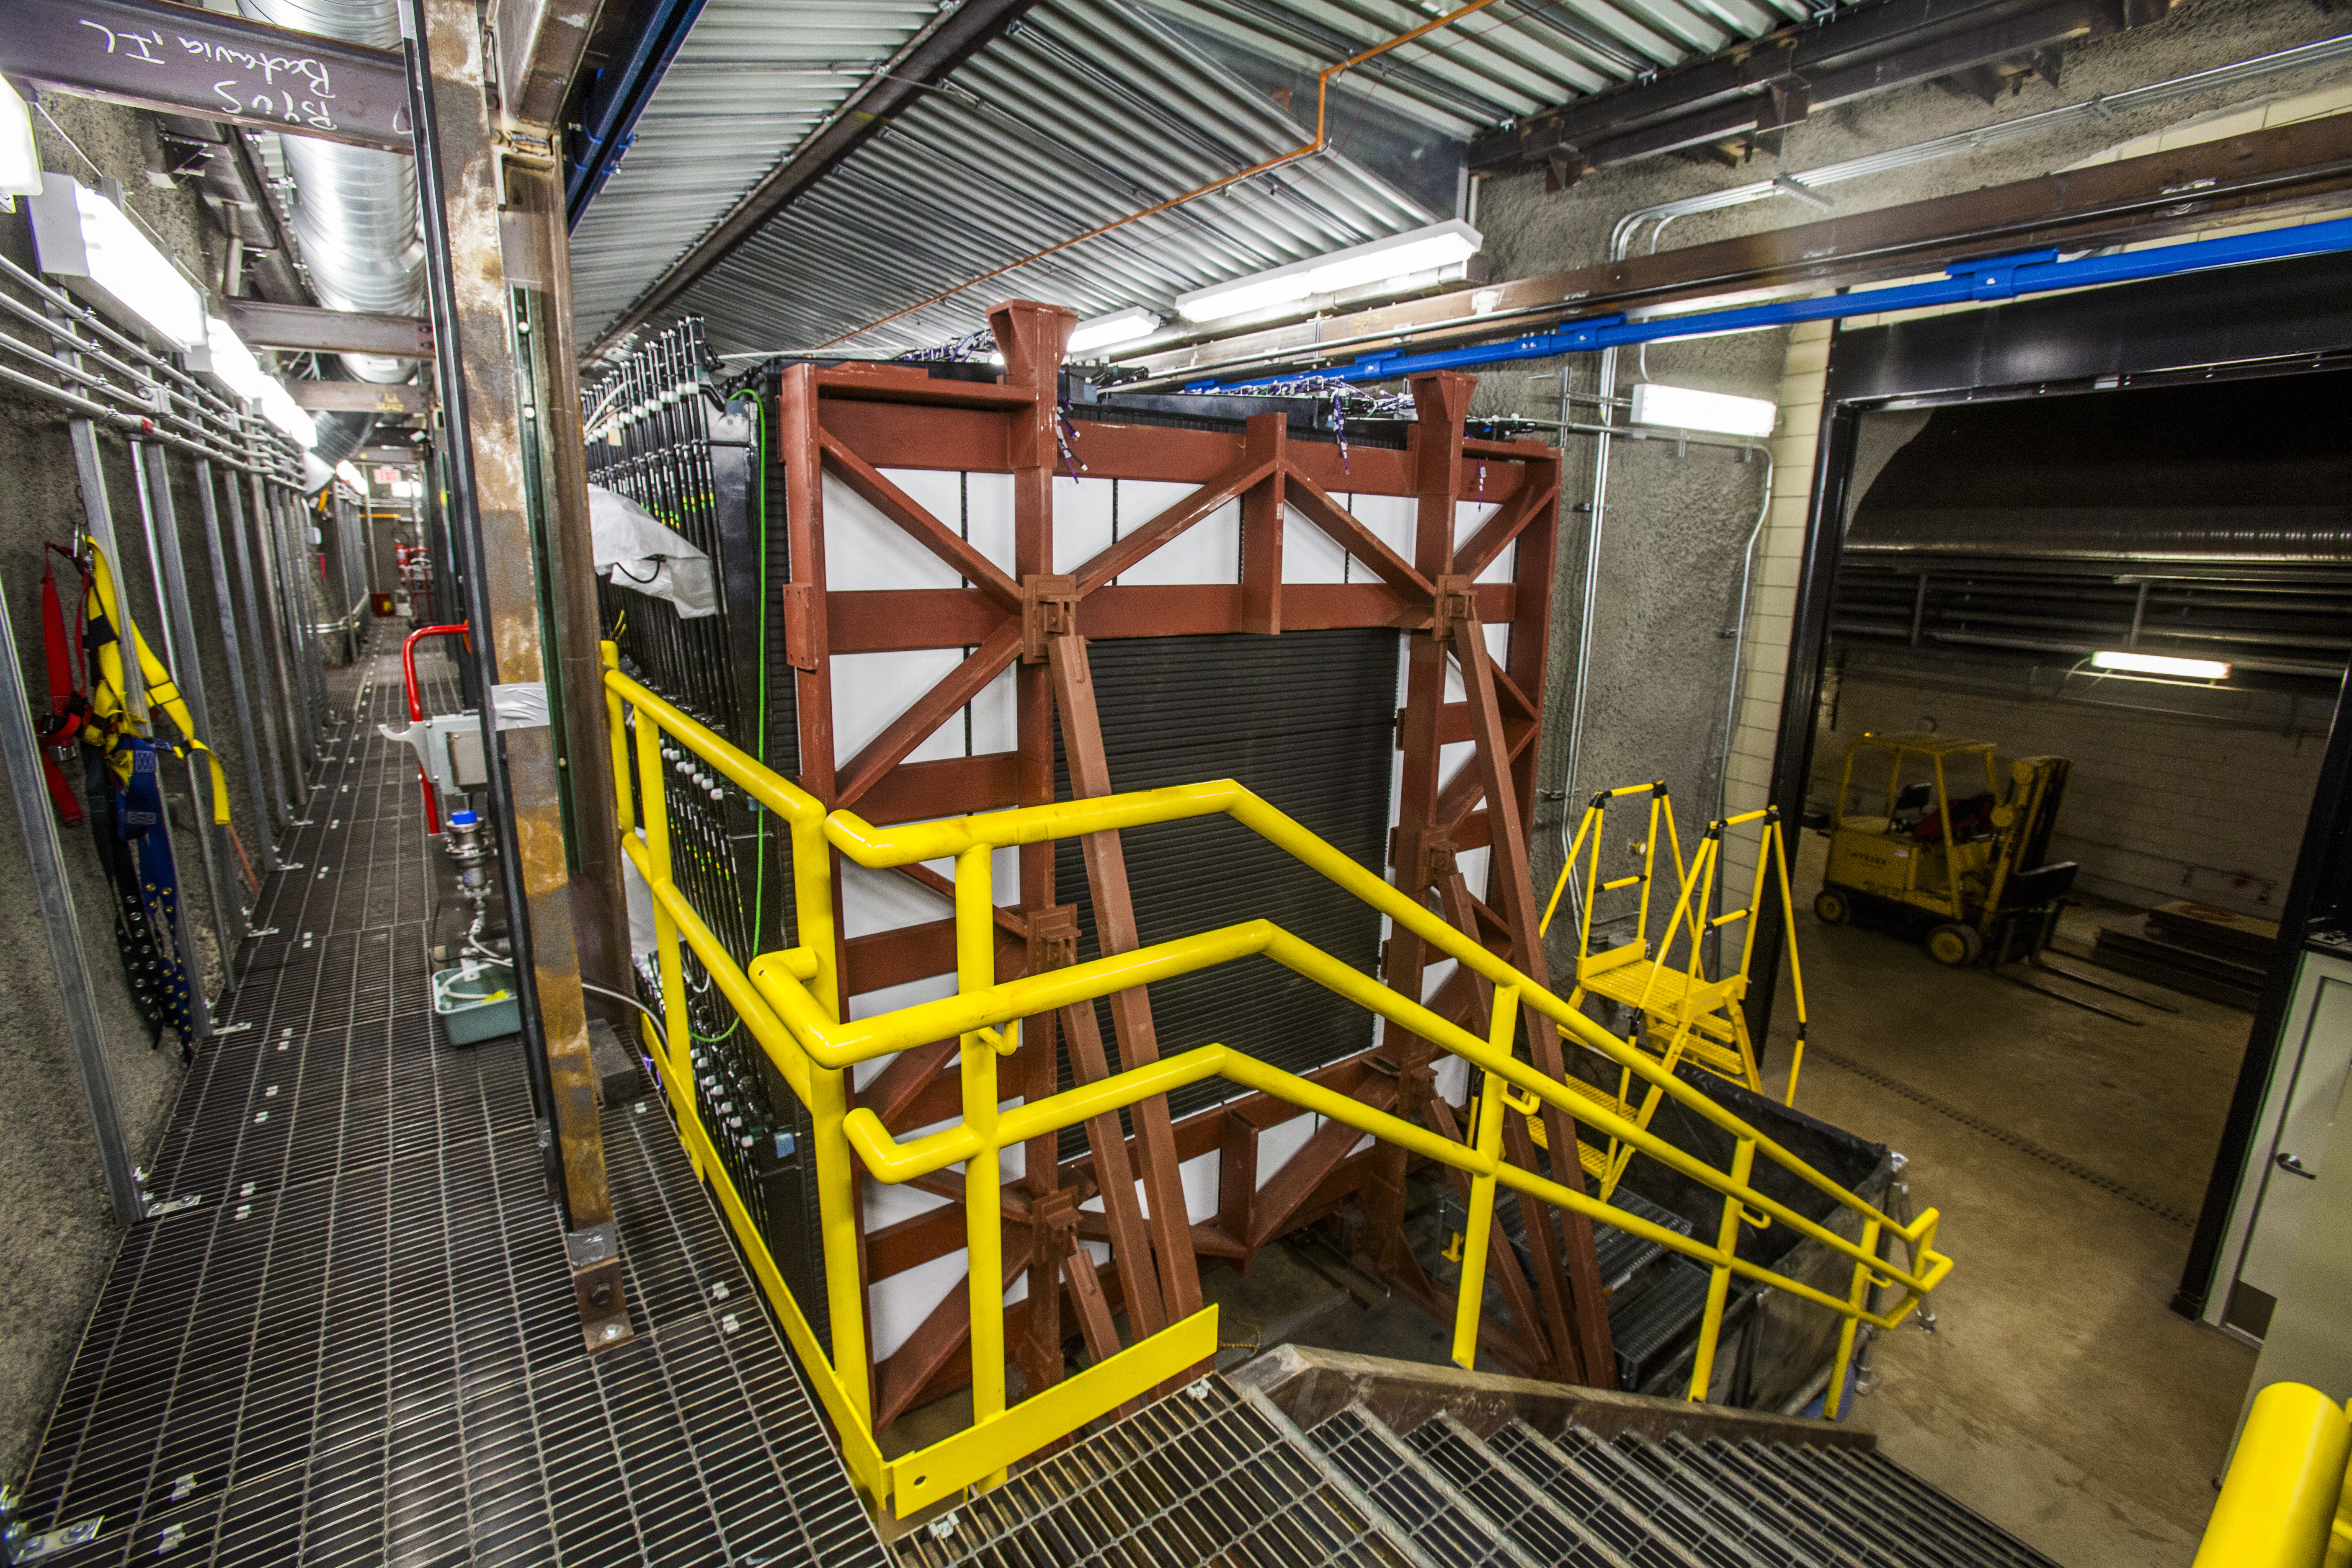
\includegraphics[height=0.55\textwidth]{figures/det_photos/ND.jpg} \end{figure}
}


\frame
{
  \frametitle{Near Detector}
	\begin{figure} \includegraphics[height=0.55\textwidth]{figures/det_photos/meND_small.jpg} \end{figure}
}

\frame
{
  \frametitle{Event Topologies}

 \begin{figure} \includegraphics[width=0.9\textwidth]{figures/figures/event_topology_nue.pdf} \end{figure}
  \vspace{-15pt}
 \begin{center}
 \footnotesize Electromagnetic radiation length is $\sim$38 cm, \\
 spans several cells (4 cm $\times$ 6 cm)
 \end{center}

}

\frame
{
  \frametitle{Event Topologies}
\begin{columns}[]
\column{0.45\textwidth}
\begin{itemize}
\item Analysis signal: \numu charged-current events
\gap
\item Muon present
\gap
\item Hadron shower topology varies
\end{itemize}
\column{0.55\textwidth}
 \begin{figure} \includegraphics[width=\textwidth]{figures/figures/event_topology_numu.pdf} \end{figure}

\end{columns}

}


\frame
{
  \frametitle{Real Far Detector Data}

 \begin{figure} \includegraphics[width=0.85\textwidth]{figures/evd_steps/evd_top_side.png} \end{figure}
 \centering \footnotesize $~$

}

\frame
{
  \frametitle{Real Far Detector Data}

 \begin{figure} \includegraphics[width=0.85\textwidth]{figures/evd_steps/evd_beam_dir.png} \end{figure}
 \centering \footnotesize Analysis uses over 10 million beam spills, $\sim 2$ min exposure,  100 kHz cosmic ray rate
}

\frame
{
  \frametitle{Real Far Detector Data}

 \begin{figure} \includegraphics[width=0.85\textwidth]{figures/evd_steps/evd_beam_dir_nu.png} \end{figure}

 \centering \footnotesize $~$

}

\frame
{
  \frametitle{Real Far Detector Data}

 \begin{figure} \includegraphics[height=0.85\textwidth, angle=-90]{figures/evd_steps/evd_oneslicehit.pdf} \end{figure}
  \centering \footnotesize $~$


}


\frame{
\frametitle{Oscillation Analysis}
\begin{tikzpicture}[]
   % Place nodes
   \node [block] (reco) {Reconstruction};
    \node [block, right = 2.7cm, right of=reco] (energy) {Energy Estimation};
   \node [block, right = 2.7cm, right of=energy, fill=emerald] (sel) {Event Selection};
    \node [block, below = 1.0cm, below of=sel] (nd) {Near Detector Data};
    \node [block, below = 2.5cm, below of=nd] (fd) {Far Detector Data};
   \node [block, left = 2.7cm, left of=nd] (eff) {Extrapolation};
   \node [block, left = 2.7cm, left of=eff] (extrap) {Prediction \\ \footnotesize{Function of oscillation parameters}};
%   \node [cloud, below =-0.5cm, below of=extrap] (fit) {Likelihood Fit};
\node[inner sep=0cm, below =2.5cm, below of=extrap, align=left] (fit)
    { \includegraphics[width=.4\textheight, angle=-90]{figures/figures/toy_spec.pdf}};
    \node [dot, right = 1.0cm, right of=sel] (bre){};
    \node [dot, right = 1.0cm, right of=fd] (brf){};
     \node [dot, right = 1.0cm, right of=nd] (brn){};

   % Draw edges
   \path [line] (reco) |- (energy);
    \path [line] (energy) |- (sel);
    \path [lin] (sel) -- (bre);
    \path [lin] (bre) -- (brf);
    \path [line] (brf) |- (fd);
    \path [line] (brn) |- (nd);
    \path [line] (nd) -- (eff);
    \path [line] (eff) -- (extrap);
    \path [line] (extrap) -- (fit);
    \path [line] (fd) -- (fit);


\end{tikzpicture}

}


\begin{frame}
\app{Reconstruction (\textit{noun})}{Extraction of patterns in raw data to aid in physics measurements}
\end{frame}


\begin{frame}

\frametitle{Reconstruction}
\framesubtitle{Slicing}

\begin{itemize}
\item First step is to resolve individual particle interactions
\gap
\item Activity is clustered in time and space to form \textit{slices}
\end{itemize}
\gap
\gap
\begin{columns}[b]
\column{0.5\textwidth}
\centering
\textcolor{custom_red}{Before Slicing}
\includegraphics[height=\textwidth, angle=-90]{figures/evd_steps/evd_hits.pdf}

\column{0.5\textwidth}
\centering
\textcolor{custom_red}{After Slicing}
\includegraphics[height=\textwidth, angle=-90]{figures/evd_steps/evd_slice.pdf}

\end{columns}

\end{frame}

\begin{frame}

\frametitle{Reconstruction}
\framesubtitle{Tracking}

\begin{itemize}
\item Tracking locates discrete particle trajectories
\end{itemize}
\gap
\gap
\gap
\begin{columns}[c]
\column{0.35\textwidth}
\centering
\includegraphics[width=\textwidth]{figures/figures/tracking.jpg}

\column{0.65\textwidth}
\centering
\includegraphics[height=\textwidth, angle=-90]{figures/evd_steps/evd_track_zoom.pdf}

\end{columns}

\end{frame}


\begin{frame}

\frametitle{Reconstruction}
\framesubtitle{Prongs}
\begin{columns}[c]
\column{0.5\textwidth}
  \begin{itemize}
  \item Prongs are for fuzzier trajectories
  \gap
  \item Primary lines are found
  \gap
  \item Vertex located using primary lines
  \gap
  \item Prongs clustered in angular space around vertex

  \end{itemize}
\column{0.5\textwidth}

\centering

\includegraphics[width=\textwidth]{figures/evd_steps/slice.png}

\includegraphics[width=\textwidth]{figures/evd_steps/hough.png}

\includegraphics[width=\textwidth]{figures/evd_steps/vertex.png}

\includegraphics[width=\textwidth]{figures/evd_steps/prongs.png}

\end{columns}


\end{frame}



\begin{frame}

\frametitle{Reconstruction}
\framesubtitle{Muon ID}
\begin{columns}[c]
\column{0.55\textwidth}
  \begin{itemize}
  \item Muons tracks can be identified
  \gap
  \item Features are extracted from tracks
    \begin{itemize}
    \item Track length
    \item Energy deposition characteristic
    \item Scattering characteristic
    \end{itemize}
  \gap
  \item Muon ID score from k-Nearest Neighbors algorithm (machine learning)
  \end{itemize}
\column{0.45\textwidth}

\centering

\includegraphics[height=\textwidth, angle=-90]{figures/plots/reco/remid_trk_len.pdf}

\includegraphics[height=\textwidth, angle=-90]{figures/plots/reco/remid_dedxll.pdf}

\end{columns}


\end{frame}


\begin{frame}
\frametitle{Energy Estimation}
\begin{columns}[c]
\column{0.55\textwidth}
  \begin{itemize}
  \item \numu CC: muon track + hadron shower
  \gap
  \item Muon energy from track length
  \gap
  \item Hadronic energy from remaining visible energy

  \end{itemize}
\column{0.45\textwidth}

\centering

\includegraphics[height=\textwidth, angle=-90]{figures/plots/reco/numu_energy_muon_fit.pdf}

\includegraphics[height=\textwidth, angle=-90]{figures/plots/reco/numu_energy_had_fit.pdf}

\end{columns}


\end{frame}

\begin{frame}
\app{Event Selection (\textit{noun})}{Identification of interaction events which display some physics signal}
\gap
\end{frame}



\begin{frame}
\frametitle{Event Classification and Selection}

\begin{itemize}
\item Goal: analyze \numu charged-current (CC) interaction events
\gap
\item Two primary sources of background must be minimized
  \begin{itemize}
  \item Cosmic rays
  \item Other $\nu$ interactions from beam, i.e. NC and \nue CC
  \end{itemize}
\end{itemize}
\end{frame}

\begin{frame}
\frametitle{Event Classification and Selection}

\begin{itemize}
\item Traditionally, classification is achieved using reconstructed features
   \begin{itemize}
  \item Criteria based on track length and other characteristics (e.g. Muon ID)
  \item Or, apply machine learning with those features
  \end{itemize}
\gap
\item But perfect reconstruction is difficult!
\gap
\item Using raw detector output could be more robust
\end{itemize}
\end{frame}


\begin{frame}
\frametitle{\nova Events as Images}

\begin{columns}[b]
\column{0.5\textwidth}

\centering
\begin{itemize}
\item \nova events are just images
  \begin{itemize}
  \item[] (two really, $X$-view and $Y$-view)
  \end{itemize}
\gap
\item Discrete pixels
\gap
\item Grayscale intensity
\end{itemize}
\vspace{20pt}
\includegraphics[width=0.85\textwidth]{figures/cnn/view_truetype6_caltype6_event155_x.pdf}


\column{0.5\textwidth}
\centering
\includegraphics[width=0.85\textwidth]{figures/cnn/view_truetype2_caltype2_event274_x.pdf}

\vspace{-5pt}


\includegraphics[width=0.85\textwidth]{figures/cnn/view_truetype13_caltype6_event144_x.pdf}

\end{columns}
\end{frame}


\begin{frame}
\frametitle{Neural Networks}

\begin{itemize}
\bang A neural network is a ``feedforward graph" of layers
  \begin{itemize}
  \item Each node, receives input \textit{only} from nodes in previous layers

  \end{itemize}
\gap
  \item Input layer: Example data to be classified
  \item Hidden layers: do the classification
  \item Output layer: classification result

\end{itemize}
\vspace{30pt}
\begin{columns}[c]
\column{0.5\textwidth}

  \begin{itemize}
  \item Supervised learning: network trained using labeled examples
  \gap
  \item ``Backpropagation": gradient-based minimization
    \begin{itemize}
    \item Network parameters are iteratively adjusted to minimize error
    \end{itemize}
  \end{itemize}
\column{0.5\textwidth}
\begin{columns}[c]
\column{0.3\textwidth}
\centering \footnotesize
Input Layer
\column{0.3\textwidth}
\centering \footnotesize
Hidden Layer
\column{0.3\textwidth}
\centering \footnotesize
Output Layer
\end{columns}
\centering
\includegraphics[width=1\textwidth]{figures/figures/basicNN.png}
\end{columns}


\end{frame}


\begin{frame}
\frametitle{Neural Networks}
  \begin{itemize}
  \bang Artificial neural networks (ANN) do well for classification of small images
    \begin{itemize}
    \item e.g. optical character recognition (OCR)
    \end{itemize}
  \end{itemize}
\begin{center}
  \includegraphics[width=0.6\textwidth]{figures/figures/ocr_ann.png}
\end{center}
\begin{itemize}
    \item But this doesn't scale well above $\sim100$ pixels

\end{itemize}

\end{frame}

\begin{frame}
\frametitle{Neural Networks}

  \begin{itemize}
  \item Image processing community harnessing new technology
    \begin{itemize}
    \item Convolutional neural networks: good for images
    \item New training strategies: deeper networks, less overtraining
    \item GPU acceleration
    \end{itemize}
  \end{itemize}

\end{frame}

\begin{frame}
\frametitle{Convolutional Layers}


  \begin{itemize}
  \item Convolutional layers work well for image classification
  \end{itemize}
  \begin{columns}[c]
  \column{0.5\textwidth}
  \centering \includegraphics[width=0.7\textwidth]{figures/figures/conv3d.png}
  \column{0.5\textwidth}
  \centering \includegraphics[width=0.7\textwidth]{figures/figures/conv.png}
  \end{columns}
  \begin{itemize}
  \gap
  \item Convolutional filters are trained to find features in patches of the image
  \gap
  \item Filters are scanned over the input image to produce a feature map
    \begin{itemize}
    \item Upshot: position independent feature extraction
    \end{itemize}
  \gap
  \end{itemize}

\end{frame}

\begin{frame}
\frametitle{Pooling Layers}
\begin{itemize}
  \item Pooling is a common down-sampling technique
\gap
  \item ``Max pooling" extracts the maximum filter output from each patch
\end{itemize}
\gap
\gap
\centering
 \includegraphics[width=0.5\textwidth]{figures/figures/pooling.png}
\end{frame}


\begin{frame}
\frametitle{Convolutional Networks}
\begin{itemize}
  \item Many filters trained in a each convolutional layer
  \gap

  \begin{center}
 \includegraphics[width=0.8\textwidth]{figures/figures/convnet.png}
 \end{center}

\end{itemize}
\end{frame}

\begin{frame}
\frametitle{GoogLeNet and \textit{Inception}}

  \begin{itemize}
  \item GoogLeNet introduced the ``Inception module"
  \end{itemize}
  \begin{center}
 \includegraphics[width=0.6\textwidth]{figures/figures/inception/inception.pdf}
 \end{center}
   \begin{itemize}
  \item Convolutional layers are arranged side-by-side rather one after another
  \item Downstream layers simultaneously learn structure at different scales
  \item $1\times1$ convolution is a tool for dimensionality reduction
    \begin{itemize}
    \item $1\times1$ convolution: constant scale factor
    \item Output filters are linear combinations of input filters
    \end{itemize}
  \end{itemize}

\end{frame}



\begin{frame}

\frametitle{\nova CNN Architecture}

  \begin{columns}
  \column{0.28\textwidth}
   \includegraphics[height=0.95\textheight]{figures/arch/arch.pdf}
  \column{0.72\textwidth}
  \begin{itemize}
  \item Separate branches for $X$ and $Y$ views
  \gap
  \item Repeated convolution, pooling, inception structures
  \gap
  \item Local Response Normalization (LRN) for smoothing
  \end{itemize}
  \end{columns}
\end{frame}

\begin{frame}
\frametitle{CNN Filter}

\begin{itemize}
\item First convolution layer, $7\times7$
\end{itemize}

\begin{columns}[b]
\column{0.45\textwidth}
\centering
\includegraphics[width=\textwidth]{figures/cnn/conv1y.pdf}

Filters
\column{0.55\textwidth}
\centering
\includegraphics[width=\textwidth]{figures/cnn/feat1_truetype2_caltype2_event274_y.pdf}

Filtered output
\end{columns}

\end{frame}


\begin{frame}
\frametitle{Inception Module Filters}

\begin{columns}[t]

\column{0.5\textwidth}
\includegraphics[width=1\textwidth,viewport=10 13 170 115, clip=true]{figures/cnn/featurePlotNuMuDIS}
\gap

\includegraphics[width=1\textwidth,viewport=10 13 170 115, clip=true]{figures/cnn/featurePlotNuMuQE}


\column{0.5\textwidth}
\includegraphics[width=1\textwidth,viewport=10 13 170 115, clip=true]{figures/cnn/featurePlotNC}
\gap
\gap
\begin{itemize}
\item Output from inception module is more discerning
\item Two particular filters in each pane
\item Top finds hadronic shower
\item Bottom finds muon tracks
\end{itemize}


\end{columns}
\end{frame}


\begin{frame}

\frametitle{CNN Softmax Output}

  \begin{center}
\includegraphics[height=0.7\textwidth, angle=-90]{figures/cnn/numu_pid_dist.pdf}

  \end{center}
  \begin{itemize}
  \item Strong discriminant for \numu CC events
  \end{itemize}
\end{frame}


\begin{frame}
\frametitle{Event Selection}

\begin{itemize}
\item Event selection serves two purposes:
  \begin{itemize}
  \item Quality: need sufficient information to estimate energy
  \item Background rejection: need clean sample of \numu CC
  \end{itemize}
\item Containment is important for both purposes
  \begin{itemize}
  \item Events which escape detector have missing energy
  \item Cosmic rays commonly traverse entire detector (i.e. touch edges)
  \end{itemize}
\end{itemize}
\begin{center}
 \includegraphics[width=0.7\textwidth]{figures/selection/cosmicmuons.png}
\end{center}

\end{frame}

\begin{frame}
\frametitle{Background Rejection}

\begin{itemize}
\item CNN output handles beam background well; also most cosmic rays
\gap
\item A few additional criteria for cosmic-ray background
\begin{itemize}
\item CosmicTrack Max-Y
\item Transverse momentum estimated from slice
\item Transverse momentum estimated from prongs
\end{itemize}
\end{itemize}

\includegraphics[height=0.5\textwidth, angle=-90]{figures/selection/n1_cvnnumu.pdf}
\includegraphics[height=0.5\textwidth, angle=-90]{figures/selection/n1_cosStartY.pdf}

\end{frame}


\begin{frame}
\frametitle{Selection Comparison}

\begin{columns}
  \column{0.5\textwidth}
  \begin{center}
   \includegraphics[height=\textwidth, angle=-90]{figures/selection/cosmic_sig_osc.pdf}
  \end{center}

  \column{0.5\textwidth}
  \begin{center}
   \includegraphics[height=\textwidth, angle=-90]{figures/selection/cosmic_sig_eff_osc.pdf}
  \end{center}

\end{columns}
\gap
  \begin{itemize}
  \item Existing \nova analysis uses muon ID and boosted decision tree (BDT)
  \gap
  \item New CNN-based selection is more efficient, especially in low energy region
  \end{itemize}
\end{frame}

\begin{frame}
\app{Analysis (\textit{noun})}{Measurement of physical parameters by comparing data to prediction}
\end{frame}


\begin{frame}
\frametitle{Analysis}
\begin{center}
\vspace{-10pt}
\includegraphics[angle=-90, width=0.45\textwidth]{figures/systs/prediction/fd_extrap_prediction_full_syst_mock_data.pdf}
\includegraphics[angle=-90, width=0.45\textwidth]{figures/systs/prediction/fd_extrap_contour_full_syst.pdf}
\end{center}


\begin{itemize}

\item FD prediction is fit to observed spectrum
\item Log-likelihood for binned, Poisson distributed data
\end{itemize}
\begin{columns}[c]
\column{0.05\textwidth}
~
\column{0.4\textwidth}
\vspace{-5pt}
\begin{equation*}
\chi^2 = 2 \sum_i e_i - o_i + o_i\ln \big (\frac{o_i}{e_i} \big)
+ \sum_j \frac{s_j^2}{\sigma_j^2}
\end{equation*}
\vspace{-5pt}
\begin{equation*}
e_i = e_i(\sin(\theta_{23}), ~\Delta m_{32}^2,~\vec{s} )
\end{equation*}
\column{0.5\textwidth}
  \begin{itemize}
  \item[] ~
  \vspace{-15pt}
  \begin{itemize}
  \item Bins: $i$
  \item Prediction in each bin: $e_i$
  \item Observation in each bin: $o_i$
  \item Systematic uncertainties: $j$
  \item Systematic shifts: $s_j$
  \item Systematic constraint: $\sigma_{ij}$
  \end{itemize}
  \end{itemize}
\end{columns}
\end{frame}

\begin{frame}
\frametitle{Prediction}
\begin{columns}[c]
\column{0.5\textwidth}
\begin{itemize}
\item FD prediction is extrapolated from ND data
\gap
\item ND data controls systematic uncertainties, e.g. flux
\gap
\item ND and FD spectra are not identical (geometric effects)
\end{itemize}
\column{0.5\textwidth}
\includegraphics[angle=-90, width=1\textwidth]{figures/plots/extrap/fd_nd_spec.pdf}


\includegraphics[angle=-90, width=1\textwidth]{figures/plots/extrap/fd_nd_ratio.pdf}

\end{columns}

\end{frame}

\begin{frame}
\frametitle{Extrapolation}

  \begin{itemize}
  \item Extrapolation also accounts for energy resolution (smearing)
  \item Reco/true matrix reweights between reconstructed and true spectra

  \end{itemize}
  \gap
  \begin{center}
   \includegraphics[width=\textwidth]{figures/figures/extrap_schematic.png}
  \end{center}
\end{frame}


\begin{frame}
\frametitle{Systematic Uncertainties}
\begin{itemize}
\item Systematic effects shift prediction
\item Events can be reweighted or energy estimate can be shifted
\item Two forms:
  \begin{itemize}
  \item Absolute: correlated between detectors (cancels well)
  \item Relative: not correlated between detectors (doesn't cancel well)
  \end{itemize}
\end{itemize}
\gap
\begin{center}
\small
\begin{tabular}{ l | l }
 \textcolor{custom_red}{Uncertainty} & \textcolor{custom_red}{Shift} \\ \hline
Flux & True energy bin reweight \\ \hline
Cross section & Event reweight for each model uncertainty \\ \hline
Particle propagation & 1\% absolute energy scale  \\
&  1\% absolute normalization scale \\ \hline
Scintillator nonlinearity & 2\% energy scale (absolute and relative)  \\
&  2\% normalization scale (absolute and relative) \\ \hline
Calorimetric energy & 2\% energy scale (absolute and relative)  \\
&  2\% normalization scale (absolute and relative) \\ \hline
Detector mass &  1\% normalization scale (absolute and relative) \\ \hline
Muon track length &  FD: 0.7\% scale on track component of energy\\
 &  ND: 2\% scale on track component of energy\\ \hline
Hadronic energy scale &  12\% scale on hadronic component of energy \\
& (absolute and relative)\\
\end{tabular}

\end{center}


\end{frame}


\begin{frame}
\frametitle{Total Uncertainty}
\begin{columns}[t]
\column{0.5\textwidth}
\centering
\textcolor{custom_red}{FD MC Prediction}
\vspace{-10pt}

\includegraphics[angle=-90, width=0.85\textwidth]{figures/systs/prediction/fd_mc_prediction_full_syst.pdf}
\vspace{15pt}
\textcolor{custom_red}{Extrapolated FD Prediction}
\vspace{-10pt}

\includegraphics[angle=-90, width=0.85\textwidth]{figures/systs/prediction/fd_extrap_prediction_full_syst.pdf}

\column{0.5\textwidth}
\centering
\textcolor{custom_red}{ND MC Prediction and Data}
\vspace{-10pt}

\includegraphics[angle=-90, width=0.85\textwidth]{figures/systs/prediction/nd_mc_prediction_full_syst.pdf}

\vspace{15pt}
\textcolor{custom_red}{90\% Confidence Interval}
\vspace{-10pt}

\includegraphics[angle=-90, width=0.85\textwidth]{figures/systs/prediction/fd_extrap_contour_full_syst.pdf}


\end{columns}



\end{frame}

\begin{frame}
\app{Result (\textit{noun})}{An item of information obtained by experiment or some other scientific method}
\end{frame}


\begin{frame}
\frametitle{Results}
\centering
Analyzed 2.74$\times 10^{20}$ POT (14 kt equivalent) -- 7\% of \nova design exposure
\gap

\begin{tabular}{c c }
 \textcolor{custom_red}{Scenario} & \textcolor{custom_red}{Prediction (events)} \\ \hline
Without oscillation & 222.0 \\
Maximal mixing & 38.1 \\ \hline
Observed & 39

\end{tabular}

\includegraphics[angle=-90,width=0.7\textwidth]{figures/results/fd_data_mc_numi_plots/ccE_unblind_wUnosc.pdf}

\end{frame}


\begin{frame}
\frametitle{Selected Event Display}
\includegraphics[angle=-90, width=1\textwidth]{figures/results/evd/evd_xzyx-proj_17953_256887.pdf}
\end{frame}

\begin{frame}
\frametitle{Selected Event Display}
\includegraphics[angle=-90, width=1\textwidth]{figures/results/evd/evd_xzyx-proj_18791_765587.pdf}
\end{frame}

\begin{frame}
\frametitle{Selected Event Display}
\includegraphics[angle=-90, width=1\textwidth]{figures/results/evd/evd_xzyx-proj_15470_124284.pdf}
\end{frame}



\begin{frame}
\frametitle{Fit}
\begin{columns}[c]
 \column{0.5\textwidth}
 \centering
 \textcolor{custom_red}{Spectrum}

  \includegraphics[angle=-90, width=1\textwidth]{figures/results/spectrum_fit_systs.pdf}
 \column{0.5\textwidth}
 \centering
  \textcolor{custom_red}{90\% Confidence Region}

  \includegraphics[angle=-90, width=1\textwidth]{figures/results/fd_extrap_contour_full_syst.pdf}
\end{columns}
\gap
\begin{itemize}
\item Selected spectrum pulls toward non-maximal mixing
\item Fit is not confident at 90\%, especially with systematics
\item Best fit:
  \begin{itemize}
  \item $\sin^2(\theta_{23}) = 0.43$
  \item $|\Delta m^2_{32}| = 2.48\times10^{-3}~\text{eV}^2$.
  \end{itemize}
\end{itemize}
\end{frame}

\begin{frame}
\frametitle{Comparison}
\centering
\includegraphics[angle=-90, width=0.9\textwidth]{figures/results/fd_extrap_contour_OverlayT2KMINOS.pdf}
\end{frame}



\begin{frame}
\frametitle{Conclusion}
\begin{itemize}
\item Neutrinos provide an important window on the universe
  \begin{itemize}
  \item Neutrino mass is beyond the standard model
  \item CP violation could explain matter/antimatter asymmetry
  \end{itemize}
\gap
\item \nova studies neutrino oscillation with a beam and two detectors
\gap
\item Convolutional neural network event classifier outperforms traditional reconstruction-based methods
\gap
\item Results are compelling, despite using just 7\% of \nova design exposure
\end{itemize}

\end{frame}

\begin{frame}
\frametitle{Future Sensitivity}
\centering
\textcolor{custom_red}{90\% Confidence Region, 6 Year Design Exposure}
\vspace{-15pt}
\includegraphics[angle=-90, width=0.85\textwidth]{figures/results/contours6yr.pdf}

\end{frame}

\appendix
\begin{frame}
\centering \huge \textcolor{custom_red}{Backup}
\end{frame}
\frame
{
  \frametitle{Oscillation in Matter}
  \framesubtitle{Interactions}
  \begin{itemize}
  \bang In the presence of matter, neutrinos can undergo coherent scattering
  \begin{columns}[c]
  \column{0.3\textwidth}
    \centering
    \includegraphics[width=\textwidth, angle=-90]{figures/feynman/ncElec.pdf}
   \column{0.3\textwidth}
      \centering
      \includegraphics[width=\textwidth, angle=-90]{figures/feynman/ncHad.pdf}
   \column{0.3\textwidth}
      \centering
      \includegraphics[width=\textwidth, angle=-90]{figures/feynman/ccElec.pdf}

\end{columns}
\bang The neutral-current scatterings affect $\nu_e$, $\nu_\mu$ and $\nu_\tau$ equally and do not affect oscillation probabilities
\bang The charged-current interaction only occurs for $\nu_e$

\end{itemize}
}
\frame
{
  \frametitle{Oscillation in Matter}
\begin{itemize}
  \framesubtitle{Effective potential}
\bang The $\nu_e$ charged-current interaction gives rise to an effective potential:
\begin{equation*}
V_{CC} = \sqrt{2}G_F n_e
\end{equation*}
\bang The effective potential modifies the $\sin$ term in the oscillation probability:
\begin{equation*}
\sin\bigg(\frac{\Delta m_{\alpha\beta}^2}{2E}L\bigg) \rightarrow
\frac{\Delta m_{\alpha\beta}^2}{\Delta m_{\alpha\beta}^2 \pm E V_{CC}/2} \sin\bigg(\big(\frac{\Delta m_{\alpha\beta}^2}{2E} \pm \frac{EV_{CC}}{2}\big)L \bigg)
\end{equation*}
\bang The $\pm$ corresponds to neutrinos/antineutrinos
  \end{itemize}
}

\begin{frame}

\frametitle{Slicing}

\begin{itemize}
\item First step is to resolve individual particle interactions
\gap
\item Use DBSCAN for clustering, A.K.A. slicing
\gap
\item Each hit pair assigned a neighbor score with time/space distance metric
\begin{equation*}
L = \bigg( \frac{\Delta t - \Delta \vec{r} / c }{T} \bigg)^2 +
     \bigg( \frac{\Delta \vec{r}}{D} \bigg)^2
\end{equation*}
\begin{center}
 ($D$ and $T$ are configurable, $c$ is speed of light)
\end{center}
\end{itemize}

\begin{columns}[c]
\column{0.3\textwidth}

\centering

\includegraphics[width=\textwidth]{figures/figures/dbscan.png}

\column{0.7\textwidth}
\begin{itemize}
\gap
\item Pairs with score below threshold start a cluster
\gap
\item Cluster boundaries formed in low density regions

\end{itemize}

\end{columns}

\end{frame}



\begin{frame}
\frametitle{Calibration}
\includegraphics[width=0.5\textwidth]{figures/plots/reco/calib_totfit_data_inX_419_219}
\includegraphics[width=0.5\textwidth]{figures/plots/reco/calib_dEdX.png}

\begin{itemize}
\item Calibration uses muons
\item Attenuation fits handle cell-to-cell and attenuation
\item Stopping muons set absolute energy scale
\end{itemize}
\end{frame}


\begin{frame}
\frametitle{Regularization}

\begin{itemize}
\item Jitter
\gap
\item Mirroring
\gap
\item Dropout in softmax layer
\gap
\item Weight penalty

\end{itemize}
\end{frame}



\frame
{
  \frametitle{Before Clustering}

 \begin{figure} \includegraphics[height=0.9\textwidth, angle=-90]{figures/evd_steps/evd_hits.pdf} \end{figure}
}

\frame
{
  \frametitle{After Clustering}

 \begin{figure} \includegraphics[height=0.9\textwidth, angle=-90]{figures/evd_steps/evd_slice.pdf} \end{figure}
}


\frame
{
  \frametitle{Neutrino Hypothesis and Discovery}

  \begin{columns}[c]
  \column{0.5\textwidth}
  \centering
  \includegraphics[height=0.37\textheight]{figures/figures/betaPretty.png}
  \column{0.5\textwidth}
  \centering
  \includegraphics[height=0.37\textheight]{figures/figures/betaspec.jpg}
  \end{columns}
  \gap
  \begin{itemize}
  \bang Beta decay originally ($\sim$1900) seen as two body decay: $p \rightarrow n + e^-$
  \bang Conservation of momentum predicts single-valued energy spectrum for $e^-$
  \bang The spectrum they measured was in fact continuous
  \vspace{10pt}
  \bang Wolfgang Pauli postulated an unseen third particle
  \bang Enrico Fermi dubbed it neutrino, or ``little neutral one"
  \bang Neutrinos from nuclear reactors were experimentally observed in 1956
  \end{itemize}
}

\begin{frame}
\frametitle{Neural Networks}

\begin{itemize}
\bang A neural network is a ``feedforward graph" of layers, $i$
  \begin{itemize}
  \item Each node,  receives input only from previous layers
  \item Nodes take input from each node in previous layer
  \item Each node passes linear combination of inputs, $z$, through a nonlinearity, $g$
  \bong \[ z_{ij} = \sum_j w_{ij} a_{(i-1)j}; ~~~~~~~~ a_{ij}  = g(z_{ij}) \]
  \end{itemize}
\end{itemize}
\vspace{20pt}
\begin{columns}[c]
\column{0.5\textwidth}

  \begin{itemize}
  \item Input layer: pixels from image
  \item Hidden layers: do the classification
  \item Output layer: classification result
  \gap
  \item Networks trained using ``backpropagation"
    \begin{itemize}
    \item Classification error is minimized in training
    \item Gradient propagated to upstream layers
    \end{itemize}
  \end{itemize}
\column{0.5\textwidth}
\centering
\includegraphics[width=1\textwidth]{figures/figures/basicNN.png}
\begin{columns}[c]
\column{0.3\textwidth}
\centering \footnotesize
Input Layer
\column{0.3\textwidth}
\centering \footnotesize
Hidden Layer
\column{0.3\textwidth}
\centering \footnotesize
Output Layer
\end{columns}
\end{columns}


\end{frame}


\begin{frame}
\frametitle{Flux Uncertainty}
\begin{columns}[b]
\column{0.5\textwidth}
\includegraphics[width=1\textwidth]{figures/systs/params/beam_had_band_nd.pdf}

\includegraphics[width=1\textwidth]{figures/systs/params/beam_had_band_fd.pdf}
\column{0.5\textwidth}
\begin{itemize}
\item Flux uncertainty is reweighted in bins of true energy
\item Left: top is ND, bottom is FD
\item Uncertainty mostly cancels in ratio, below
\end{itemize}
\gap
\gap
\includegraphics[width=1\textwidth]{figures/systs/params/beam_had_band_fd_nd_ratio.pdf}

\end{columns}

\end{frame}

\begin{frame}
\frametitle{Particle Propagation Uncertainty}

\begin{columns}[c]

\column{0.4\textwidth}

\includegraphics[angle=-90, width=1\textwidth]{figures/systs/params/nd_QGSP_BIC_HP.pdf}

\column{0.6\textwidth}

\begin{center}
\small
\begin{tabular}{|l|c|c|}
\hline
Physics List & Mean Ratio & Norm. Ratio \\ \hline
FTFP\_BERT  &  0.999 & 1.001\\ \hline
FTF\_BIC &  0.994 & 1.008  \\ \hline
QGSC\_BERT  &  0.998 & 0.999\\ \hline
QGSP\_BIC\_HP  &  0.991 & 0.993\\ \hline
\end{tabular}
\end{center}




\end{columns}

\begin{itemize}
\item Alternative samples generated with different physics lists
\item Beam peak fit with normal distribution
\item Ratio of fit mean and normalization used to parameterize mean and normalization shift
\end{itemize}



\end{frame}

\begin{frame}
\frametitle{Scintillation Production Uncertainty}
\begin{columns}[c]

\column{0.4\textwidth}

\includegraphics[angle=-90, width=\textwidth]{figures/systs/params/fd_birksb.pdf}

\column{0.6\textwidth}

\begin{center}
\begin{tabular}{|l|c|c|}
\hline
$k_B (\text{cm} / \text{MeV})$ & Mean Ratio & Norm. Ratio \\ \hline
$0.02 $ & 0.981 & 0.977  \\ \hline
$0.01 $ & 0.996 & 0.983  \\ \hline
\end{tabular}
\end{center}




\end{columns}

\begin{itemize}
\item Alternative samples generated with different Birks-Chou parameters
\begin{equation}
\frac{dL}{dX} = L_0  \frac{\frac{dE}{dX}}{1+ k_B \frac{dE}{dX} + k_C \frac{dE}{dX}^2}.
\end{equation}
\item Beam peak fit with normal distribution
\item Ratio of fit mean and normalization used to parameterize mean and normalization shift
\end{itemize}

\end{frame}

\begin{frame}
\frametitle{Calibration Uncertainty}

\begin{columns}[c]

\column{0.4\textwidth}


\includegraphics[angle=-90, width=1\textwidth]{figures/systs/params/fd_flat105cal.pdf}

\column{0.6\textwidth}
\begin{center}
\begin{tabular}{|l|c|c|}
\hline
Sample & Mean Ratio & Norm. Ratio \\ \hline
$+5$\% Scale & 1.020 & 0.981 \\ \hline
$-5$\% Scale& 0.980 & 1.013 \\ \hline
Random & 1.001 & 0.996 \\ \hline
Atten. slope & 1.009 & 0.995 \\ \hline
\end{tabular}
\end{center}



\end{columns}

\begin{itemize}
\item Alternative samples generated with altered calibration
\item Beam peak fit with normal distribution
\item Ratio of fit mean and normalization used to parameterize mean and normalization shift
\end{itemize}
\end{frame}


\begin{frame}
\frametitle{Detector Mass Uncertainty}
\begin{center}
\small
\begin{tabular}{|l|c|c|c|c|}
\hline
& \multicolumn{2}{c|}{FD} & \multicolumn{2}{c|}{ND} \\ \hline
Component    & Mass (kg/m/cell)   & Percentage & Mass (kg/m/cell) & Percentage \\ \hline
Extrusions   & 0.951 $\pm$ 0.016  & 36.4 $\pm$ 0.6  &  0.951 $\pm$ 0.016  & 36.2 $\pm$ 0.6 \\
Scintillator & 1.641 $\pm$ 0.009  & 62.8 $\pm$ 0.3  &  1.653 $\pm$ 0.011  & 63.0 $\pm$ 0.4 \\
Glue         & 0.019 $\pm$ 0.0003 & 0.07 $\pm$ 0.01 &  0.019 $\pm$ 0.0003 & 0.07 $\pm$ 0.01 \\
Fiber        & 0.001 $\pm$ 0.0001 & 0.04 $\pm$ 0.04 &  0.001 $\pm$ 0.0001 & 0.04 $\pm$ 0.04 \\ \hline
Total        & 2.612 $\pm$ 0.018  & 100.0 $\pm$ 0.7 &  2.624 $\pm$ 0.019  & 100.0 $\pm$ 0.07 \\ \hline
\end{tabular}
\end{center}

\begin{itemize}
\item Material uncertainties propagated
\item 1\% normalization in ND
\end{itemize}
\end{frame}


\begin{frame}
\frametitle{\nova Reach}
\begin{columns}[c]
\column{0.5\textwidth}
\centering
\textcolor{custom_red}{Hierarchy Sensitivity}

\includegraphics[width=\textwidth]{figures/plots/nova/hie_sens.pdf}
\column{0.5\textwidth}
\centering
\textcolor{custom_red}{CP Violation Sensitivity}

\includegraphics[width=\textwidth]{figures/plots/nova/cpv_sens_t2k.pdf}

\end{columns}
\begin{itemize}
\item backup slide on this
\end{itemize}
\end{frame}

\begin{frame}
\frametitle{Feldman-Cousins}
\centering
\includegraphics[angle=-90, width=0.9\textwidth]{figures/results/fc_compare.pdf}
\end{frame}


\begin{frame}

\frametitle{CNN Output}

  \begin{center}
  \includegraphics[height=0.7\textwidth, angle=-90]{figures/selection/n1_cvnnumu.pdf}

  {\footnotesize(``$n-1$'' histogram -- only events which pass all other criteria)}
  \end{center}
  \begin{itemize}
  \item Select events with CNN output > 0.5
  \end{itemize}
\end{frame}



\begin{frame}
\frametitle{CosmicTrack start $Y$ position}

  \begin{center}
  \includegraphics[height=0.7\textwidth, angle=-90]{figures/selection/n1_cosStartY.pdf}

  {\footnotesize(``$n-1$'' histogram -- only events which pass all other criteria)}
  \end{center}
  \begin{itemize}
  \item Select events with start $Y$ < 6.0 m
  \end{itemize}
\end{frame}


\begin{frame}
\frametitle{Transverse momentum from slice mean}

  \begin{center}
  \includegraphics[height=0.7\textwidth, angle=-90]{figures/selection/n1_tranMom.pdf}

  {\footnotesize(``$n-1$'' histogram -- only events which pass all other criteria)}
  \end{center}
  \begin{itemize}
  \item Select events with $P_T$ < 0.8
  \end{itemize}
\end{frame}

\begin{frame}
\frametitle{Transverse momentum from prongs}

  \begin{center}
  \includegraphics[height=0.7\textwidth, angle=-90]{figures/selection/n1_pngptp.pdf}

  {\footnotesize(``$n-1$'' histogram -- only events which pass all other criteria)}
  \end{center}
  \begin{itemize}
  \item Select events with $P_T$ < 0.8
  \end{itemize}
\end{frame}

\begin{frame}
\frametitle{Contour Improvement}
\centering
\includegraphics[angle=-90, width=0.9\textwidth]{figures/selection/contoursfhc1cosmic.pdf}
\end{frame}


\end{document}
